\chapter{OpenCAL}

With OpenCAL, we identify the sequential version of the software
library, which runs on just a single core of your CPU, and represents
the basis for the other parallel versions. Moreover, it allows for
some \emph{unsafe operations}, which can significantly speed up your
application. Such unsafe operations can also be found in the OpenMP
version, while they are not present to GPU one.

In the following sections, we will introduce OpenCAL by examples. In
the first part of the Chapter, we will deal with the OpenCAL's safe
mode, while in the last one, we will go deep inside OpenCAL,
discussing unsafe operations.

\section{Conway's Game of Life}

In order to introduce you to Cellular Automata development with
OpenCAL, we start this section by implementing the Conway's Game of
Life. It represents one of the most simple, yet powerful examples of
Cellular Automata, devised by mathematician John Horton Conway in
1970.

The Game of Life can be thought as an infinite two-dimensional
orthogonal grid of square cells (the cellular space), each of which is
in one of two possible states, dead or alive. Every cell interacts
with its eight neighbors, which are the cells that are directly
horizontally, vertically, or diagonally adjacent to it (the Moore
neighborhood). At each time step, one of the following transitions
occur:

\begin{enumerate}
    \item Any live cell with fewer than two alive neighbors dies, as
      if by loneliness.
    \item Any live cell with more than three alive neighbors dies, as
      if by overcrowding.
    \item Any live cell with two or three alive neighbors lives,
      unchanged, to the next generation.
    \item Any dead cell with exactly three live neighbors comes to
      life.
\end{enumerate}

The initial configuration of the system specifies the state (dead or
alive) of each cell into the cellular space. The evolution of the
system is thus obtained by applying the above rules (the CA transition
function) simultaneously to every cell in the cellular space, so that
each new configuration is function of the one at the previous
step. The rules continue to be applied repeatedly to create further
generations. For more details on the Game of life you can check
Wikipedia at the URL
\url{http://en.wikipedia.org/wiki/Conway's_Game_of_Life}.

The formal definition of the Life CA is reported below.

$$Life = < R, X, Q, \sigma >$$

where:

\begin{itemize}

\item $R$ is the set of points, with integer coordinates, which
  defines the 2-dimensional cellular space. The generic cell in $R$ is
  individuated by means of a couple of integer coordinates $(i, j)$,
  where $0 \leq i < i_{max}$ and $0 \leq j < j_{max}$. The firt
  coordinate, $i$, represents the row, while the second, $j$, the
  column. The cell at coodinates $(0,0)$ is located at the top-left
  corner of the computational grid.

\item $X = \{(0,0), (-1, 0), (0, -1), (0, 1), (1, 0), (-1,-1), (1,-1),
  (1,1), (-1,1)\}$ is the Moore neighborhood relation, a geometrical
  pattern which identifies the cells influencing the state transition
  of the central cell. The neighborhood of the generic cell of
  coordinate $(i, j)$ is given by
  $$N(X, (i, j)) = $$
  $$= \{(i, j)+(0,0), (i, j)+(-1, 0), \dots, (i, j)+(-1,1)\} =$$
  $$= \{(i, j), (i-1, j), \dots, (i-1,j+1)\}$$
  Here, a subscript operator can be used to index cells belonging to the
  neighbourhood. Let $|X|$ be the number of elements in X, and $n \in
  \mathbb{N}$, $0 \leq n < |X|$; the notation

  $$N(X, (i, j), n)$$

  represents the $n^{th}$ neighbourhood of the cell $(i,j)$. Thereby,
  $N(X, (i, j), 0) = (i, j)$, i.e. the central cell, $N(X, (i, j), 1)
  = (i-1, j)$, i.e. the first neighbour, and so on.
  
\item $Q = \{0, 1\}$ is the set of cell states.
  
\item $\sigma : Q^9 \shortrightarrow Q$ is the deterministic cell
  transition function. It is composed by one elementary process, which
  implements the previously descripted transition rules.
\end{itemize}


The program below shows a simple Game of Life sequential
implementation in C with OpenCAL. As you can see, even if Listing
\ref{lst:cal_life} is very short, it completely defines the Conway's
Game of Life CA and perform a simulation (actually, only one step in
this example).

\lstinputlisting[float,floatplacement=H, label=lst:cal_life, caption=An OpenCAL implementation of the Conway's game of Life.]{../opencal/OpenCAL/examples/cal_life/source/life.c}

In order to use OpenCAL, you need to include some header files (lines
3-5). Specifically, \verb'cal2D.h' (line 3) allows you to define the
CA object (line 9) and the related substate (line 10), while
\verb'cal2DRun.h' (line 5) allows you to define a CA simulation object
(line 11), needed to run the CA model. The \verb'cal2DIO.h' header
file (line 4) provides you some input/output functions for
reading/writing substates from/to file.

While statements at lines 9-11 just declare the required objects, they are
defined later in the \verb'main' function. In particular, the life CA
object is defined at line 29 by the \verb'calCADef2D()' function. The
first 2 parameters define the CA dimensions (the number of rows and
columns, respectively), while the third the neighbourhood pattern. The
fourth parameter specifies the boundary conditions. In this case, the CA
cellular space is considered as a torus, with cyclic behaviour at
boundaries. The last parameter allows you to specify if your model
has to use the so called \emph{active cells optimization}, that is
able to restrict the computation to only \emph{non-stationary cells}. In this
case, no optimization is considered.

\begin{lstlisting}[float,floatplacement=H, label=lst:calCADef2D, caption=Definition of the calCADef2D() function., numbers=none]
  struct CALModel2D* calCADef2D (
    int rows,
    int columns,
    enum CALNeighborhood2D CAL_NEIGHBORHOOD_2D,
    enum CALSpaceBoundaryCondition CAL_TOROIDALITY,
    enum CALOptimization CAL_OPTIMIZATION
  )
\end{lstlisting}  

The complete definition of \verb'calCADef2D()' is provided in Listing
\ref{lst:calCADef2D}. In particular, the \verb'CALNeighborhood2D' enum
type (Listing \ref{lst:CALNeighborhood2D}) allows you to select one of
the square or hexagonal predefined neighbourhoods, or a custom
neighbourhood, whose pattern can be defined directly in your
application. Custom neighbourhoods will be discussed later in this
Chapter. Similarly, the \verb'CALSpaceBoundaryCondition' enum type
(Listing \ref{lst:CALSpaceBoundaryCondition}) allows you to set
non-ciclic or cyclic behaviour at the boundaries of the cellular
space. Eventually, the \verb'CALOptimization' enum type (Listing
\ref{lst:CALOptimization}) allows you to use or not the active cells
optimization.

\begin{lstlisting}[float,floatplacement=H, label=lst:CALNeighborhood2D, caption=The CALNeighborhood2D enum type., numbers=none]
  enum CALNeighborhood2D { 
    CAL_CUSTOM_NEIGHBORHOOD_2D,
    CAL_VON_NEUMANN_NEIGHBORHOOD_2D,
    CAL_MOORE_NEIGHBORHOOD_2D,
    CAL_HEXAGONAL_NEIGHBORHOOD_2D,
    CAL_HEXAGONAL_NEIGHBORHOOD_ALT_2D 
};
\end{lstlisting}  

\begin{lstlisting}[float,floatplacement=H, label=lst:CALSpaceBoundaryCondition, caption=The CALSpaceBoundaryCondition enum type., numbers=none]
  enum CALSpaceBoundaryCondition{
    CAL_SPACE_FLAT = 0,         
    CAL_SPACE_TOROIDAL
  };
\end{lstlisting}

\begin{lstlisting}[float,floatplacement=H, label=lst:CALOptimization, caption=The CALOptimization enum type., numbers=none]
  enum CALOptimization{
    CAL_NO_OPT = 0,
    CAL_OPT_ACTIVE_CELLS        
  };
\end{lstlisting}

The CA simulation object is defined at line 30 by the
\verb'calRunDef2D()' function. The first parameter is a pointer to a
CA object (\verb'life' in our case), while the second and third
parameters specify the initial and last simulation step,
respectively. In this case, we just perform one step of computation,
being both the first and last step set to 1. The last parameter allows
you to specify the substate update policy. It can be implicit or
explicit. In the first case, OpenCAL does substates' updates for you,
while in the second case the substates' updates is your
responsibility. Note that, in case implicit update policy is applyied,
all the CA substates are updated after the execution of each
elementary process composing the CA transition function. We will
discuss update policies later in this Chapter. The complete definition
of \verb'calRunDef2D()' is provided in Listing
\ref{lst:calRunDef2D()}. The \verb'CALUpdateMode' type (Listing
\ref{lst:CALUpdateMode}) enumerates possible update policies.

\begin{lstlisting}[float,floatplacement=H, label=lst:calRunDef2D(), caption=Definition of the calRunDef2D() function., numbers=none]
  struct CALRun2D* calRunDef2D (
    struct CALModel2D* ca2D,
    int initial_step,
    int final_step,
    enum CALUpdateMode UPDATE_MODE 
  )	
\end{lstlisting}

\begin{lstlisting}[float,floatplacement=H, label=lst:CALUpdateMode, caption=The CALUpdateMode enum type., numbers=none]
  enum CALUpdateMode {
    CAL_UPDATE_EXPLICIT = 0,
    CAL_UPDATE_IMPLICIT
  };
\end{lstlisting}

Line 33 allocates memory and registers the substate \verb'Q' to the
\verb'life' CA, while line 36 adds an elementary process to the cell
transition function. The \verb'calAddSubstate2Di()' function is very
simple and self-explanatory. At the contrary,
\verb'calAddElementaryProcess2D()' must be discussed more in detail. It
takes the handle to the CA model to which the elementary process must
be attached and a pointer to a callback function, that defines the
elementary process itself. In our example, we specified
\verb'life_transition_function' as second parameter, being it the name
of a developer-defined function that you can find at lines 14-24. As
you can see, the elementary process callback returns
\verb'void'. Moreover, it takes a pointer to a CA object as first
parameter, followeb by a couple of integers, representing the
coordinates of the generic cell in the CA space. This is the function
prototype which is common to each elementary process you add to your
application. Note that, each elementary process is applyed by OpenCAL
simultaneously to each cell of the cellular space in a computational
step. However, this is completely transparent to the user, so that he/she
can concentrate his/her effort on the definition of single cell behaviour.

When the user is going to implement an elementary process, by defining
its callback function, he/she can rely on a set of OpenCAL functions that
allow to get the substates values of both the central and the
neighbouring cells, and to update the substates values of the central
cell. In the specific case of the Game of Life, we used the
\verb'calGet2Di()' function to get the central cell's value of the
substate \verb'Q' (remember that the central cell is identified by the
coordinates (i, j), coming from the callback parameters), the
\verb'calGetX2Di()' function to get the value of the n-th neighbour's
substate \verb'Q', and the \verb'calSet2Di()' function to update the
value of the substate \verb'Q' for the central cell. In the Game of
Life example, we defined just one elementary process, that therefore
represents the whole cell transition function. However, as we will see
later, many elementary processes can be defined in OpenCAL by simply
calling the \verb'calAddElementaryProcess2D()' function many times. If
you define more than one elementary process, they will be executed in
the order they are added to the CA.

The \verb'calInitSubstate2Di()' function at line 39 sets the whole
substate \verb'Q' to the value 0, i.e. the value of the substate
\verb'Q' is set to 0 in each cell of the cellular space. The following
lines, from 42 to 46, set the value of the substate \verb'Q' for some
cells to 1, in order to define a well known \emph{glider} pattern. In
this case, we provided the cells coordinates as the third and fourth
parameters. In this way, we define the initial condition of the system
direcly inside the \verb'main' function. However, as we will see later
in this Chapter, such kind of initialization can be performed by means
of a specific function.

The \verb'calSaveSubstate2Di()' function (line 49) saves the substate
\verb'Q' to file, while the \verb'calRun2D()' function (line 52)
enters the simulation loop (actually, only one computational step in
this example), and returns to the \verb'main' function when the
simulation is complete. The \verb'calSaveSubstate2Di()' is thus called
again at line 55 to save the new (last) configuration of the CA
(represented by the only defined substate \verb'Q') to file, while the
last two functions at lines 58 and 59 release previously allocated memory. The
\verb'return' statement at line 61 ends our first example.

Figures \ref{fig:life_0000} and \ref{fig:life_LAST} show the initial and final configuration of Game of Life as implemented in Listing \ref{lst:cal_life}, respectively.

\begin{figure}
  \begin{center}
    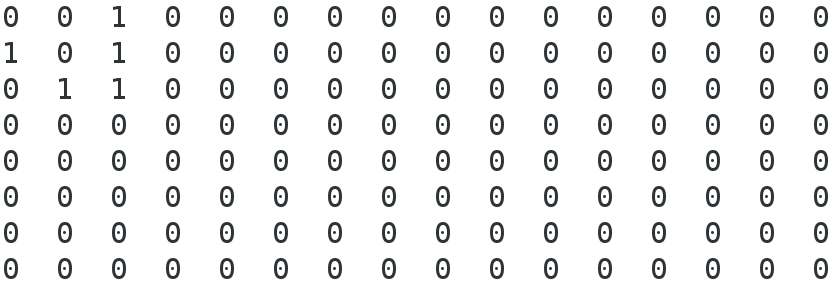
\includegraphics[width=7cm]{./images/OpenCAL/life_0000}
    \caption{Initial configuration of Game of Life, as implemented in Listing \ref{lst:cal_life}.}
    \label{fig:life_0000}
  \end{center}
\end{figure}

\begin{figure}
  \begin{center}
    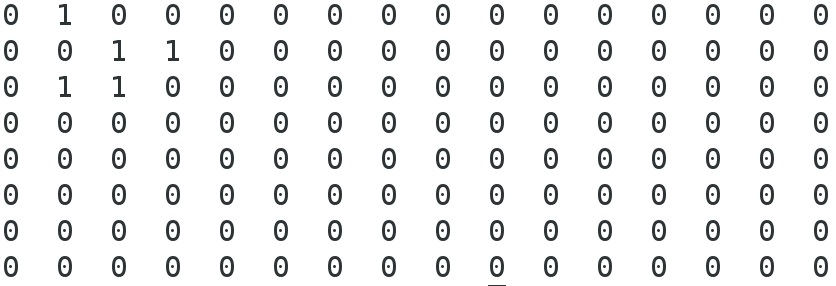
\includegraphics[width=7cm]{./images/OpenCAL/life_LAST}
    \caption{Final configuration of Game of Life (actually, just one step of computation), as implemented in Listing \ref{lst:cal_life}.}
    \label{fig:life_LAST}
  \end{center}
\end{figure}

\section{OpenCAL statement convention}
As you can easily see from a rapid sight to the source code, all the
OpenCAL statements are characterized by a prefix and a suffix. All the
data types have the \verb'CAL' prefix, and an optional suffix that
identifies the CA dimension (e.g. 2D for a two-dimensional model) and
the basic type. For instance, in the case of the Life's \verb'Q'
substate, the 2Di suffix of the \verb'CALSubstate2Di' type specifies
that it is a two-dimensional substate in whihc each element is of
integer type.

More in detail, OpenCAL comes with three different basic numeric
types, whihc are in lowercase (besides the prefix):
\begin{itemize}
\item \verb'CALbyte', corresponding to the \verb'char' C data type;
\item \verb'CALint', corresponding to the \verb'int' C data type;
\item \verb'CALreal', corresponding to the \verb'long double' C data type;
\end{itemize}
while the possible substates types are:
\begin{itemize}
\item \verb'CALSubstate2Db', corresponding to a \verb'CALbyte' based substate;
\item \verb'CALSubstate2Di', corresponding to a \verb'CALint' based substate;
\item \verb'CALSubstate2Dr', corresponding to a \verb'CALreal' based substate;
\end{itemize}
Also the OpenCAL constants have a prefix, namely the \verb'CAL_' one,
followd by at least one uppercase keyword. In case of more kewords, they
are separated by the \verb'_' character. Eventually, all the OpenCAL
functions start with the \verb'cal' suffix, followed by at least one
capitalized keyword, and end with a suffix specifying the CA dimension
and the basic datatype.


\section{SciddicaT}
In the previous section we illustrated an OpenCAL implementation of a
simple cellular automaton, namely the Conway’s Game of Life. Here, we
will deal with a more complex example concerning the implementations
of the SciddicaT Cellular Automata model for landslide
simulation. Different versions will be presented, ranging from a naiv
to a fully optimized implementation.

Sciddica is a family of bi-dimensional CCA debris flow models,
successfully applied to the simulation of many real cases, such as the
1988 Mt. Ontake (Japan) landslide and the 1998 Sarno (Italy)
disaster. An oversimplified toy-version of Sciddica (SciddicaT in the
following) was here considered to be implemented in \verb"OpenCAL",
and its application to the 1992 Tessina (Italy) landslide shown.

SciddicaT considers the surface over which the phenomenon evolves as
subdivided in square cells of uniform size. Each cell changes its
state by means of the transition function, which takes as input the
state of the cells belonging to the von Neumann neighborhood. It is
formally defined as:

$$SciddicaT = < R, X, Q , P, \sigma  >$$

where:

\begin{itemize}

\item $R$ is the set of points, with integer coordinates, which
  defines the 2-dimensional cellular space over which the phenomenon
  evolves. The generic cell in $R$ is individuated by means of a
  couple of integer coordinates $(i, j)$, where $0 \leq i < i_{max}$
  and $0 \leq j < j_{max}$. The firt coordinate, $i$, represents the
  row, while the second, $j$, the column. The cell at coodinates
  $(0,0)$ is located at the top-left corner of the computational grid.

\item $X = \{(0,0), (-1, 0), (0, -1), (0, 1), (1, 0)\}$ is the von
  Neumann neighborhood relation, a geometrical pattern which
  identifies the cells influencing the state transition of the central
  cell. The neighborhood of the generic cell of coordinate $(i, j)$ is
  given by
$$N(X, (i, j)) =$$
$$= \{(i, j)+(0,0), (i, j)+(-1, 0), (i, j)+(0, -1),
(i, j)+(0, 1), (i, j)+(1, 0)\} =$$
$$= \{(i, j), (i-1, j), (i, j-1), (i, j+1), (i+1, j)\}$$

Here, a subscript operator can be used to index cells belonging to the
neighbourhood. Let $|X|$ be the number of elements in X, and $n \in
\mathbb{N}$, $0 \leq n < |X|$; the notation

$$N(X, (i, j), n)$$

represents the $n^{th}$ neighbourhood of the cell $(i,j)$. Thereby, $N(X, (i, j), 0) = (i, j)$, i.e. the central cell, $N(X, (i, j), 1) = (i-1, j)$, i.e. the first neighbour, and so on. 
  
\item $Q$ is the set of cell states. It is subdivided in the following
  substates:

\begin{itemize}
    \item   $Q_z$ is the set of values representing the topographic altitude (i.e. elevation);
    \item   $Q_h$ is the set of values representing the debris thickness;
    \item   $Q_o^4$ are the sets of values representing the debris outflows from the central cell to the neighboring ones.
\end{itemize}

The Cartesian product of the substates defines the overall set of
state $Q$:

$$Q = Q_z \times Q_h \times Q_o^4$$
so that the cell state is specified by the following sixtuple:

$$ q = (q_z, q_h, q_{o_0}, q_{o_1}, q_{o_2}, q_{o_3})$$
In particular, $q_{o_0}$ represents the outflows from the central cell towards the neighbour 1, $q_{o_1}$ the outflow towards the neighbour 2, and so on.

\item   $P$ is set of parameters ruling the CA dynamics:

\begin{itemize}
    \item   $p_\epsilon$ is the parameter which specifies the thickness of the debris that cannot leave the cell due to the effect of adherence;
    \item   $p_r$ is the relaxation rate parameter, which affects the size of outflows (cf. section above).
\end{itemize}

\item $\sigma : Q^5 \shortrightarrow Q$ is the deterministic cell
  transition function. It is composed by two elementary processes,
  listed below in the same order they are applied:
\begin{itemize}
\item $\sigma_1 : (Q_z \times Q_h)^5 \times p_\epsilon \times
  p_r\shortrightarrow Q_o^4$ determines the outflows from the central
  cell to the neighboring ones by applying the \emph{minimization
    algorithm of the differences}. In brief, a preliminary control
  avoids outflows computation for those cells in which the amount of
  debris is smaller or equal to $p_\epsilon$, acting as a
  simplification of the adherence effect. Thus, by means of the
  minimization algorithm, outflows $q_o(0,m) \; (m=0,\ldots,3)$ from
  the central cell towards its four adjecent cells are evaluated, and
  the $Q_o^4$ substates accordingly updated. Note that, $q_o(0,0)$
  represents the aoutflow from the central cell towards the neighbour
  1, $q_o(0,1)$ the aoutflow towards the neighbour 2, and so on. In
  general, $q_o(0,m)$ represnets the outflows from the central cell
  towards the $n=(m+1)^{th}$ neighbouring cell. Eventually, a
  relaxation rate factor, $p_r \in \; ]0,1]$, is considered in order
      to obtain the local equilibrium condition in more than one CA
      step. This can significantly improve the realism of model as, in
      general, more than one step may be needed to displace the proper
      amount of debris from a cell towards the adjacent ones. In this
      case, if $f(0,m) \; (i=0, \ldots, 3)$ represent the outgoing
      flows towards the 4 adjacent cells, as computed by the
      minimization algorithm, the resulting outflows are given by
      $q_o(0,m)=f(0,m) \cdot p_r \; (i=0, \ldots, 3)$.

      %% , while the amount of debris remaining in the central cell is
      %% obtained as: $$h_r(0) = q_0(0,0) = h(0) - \sum_{i=1}^4
      %% q_4(0,i)$$

\item $\sigma_2: Q_h \times (Q_o^4)^4 \shortrightarrow Q_h$ determines
  the value of debris thickness inside the cell by considering mass
  exchange in the cell neighborhood: $h'(0) = h(0) + \sum_{m=0}^3
  (q_o(0,m) - q_o(m,0))$. Here, $h'(0)$ is the new debris
  thickness inside the cell, while $q_o(m,0)$ represents the inflow from
  the $n=(m+1)^{th}$ neighbouring cell. No parameters are involved in
  this elementary process.

\end{itemize}
\end{itemize}

In the following Listing \ref{lst:cal_sciddicaT}, an OpenCAL
implementation of SciddicaT is shown.

\lstinputlisting[label=lst:cal_sciddicaT, caption=An OpenCAL implementation of the SciddicaT debris flows simulation model.]{../opencal/OpenCAL/examples/cal_sciddicaT/source/sciddicaT.c}

As for the case of Game of Life, the CA model and the simulation
objects are declared as global variables (lines 22 and 35,
respectively), and defined later into the main function (lines 147 and
148, respevctively). As you can see, the 2D cellular space is a grid
of \verb'ROWS' rows times \verb'COLS' columns cells, corresponding to
$i_{max}$ and $j_{max}$ of the formal definition, respectively
(cf. lines 10-11), while the von Neumann neighbourhood is adopted. The
cellular space is still toroidal, as in Life, and no optimization is
considered. Regarding the simulation object, a total of \verb'STEPS'
steps (i.e. 4000 steps - cf. line 14) are set, and implicit substates
updating considered.

Substates and parameters are grouped into two different C structures
(lines 24-28 and 30-33, respectively). Substates are therefore bound to
the CA context by means of the \verb'calAddSubstate2Dr()' function
(lines 155-160), as well as elementary processes are defined as
collback functions by means of the \verb'calAddElementaryProcess2D()'
function (lines 151-152).

The topographic altitude and debris thickness substates are
initialized from files through the \verb'calLoadSubstate2Dr()'
function (lines 163-164), while the remaining initial state of the CA
is set by means of the \verb'calRunAddInitFunc2D()' function. It
registers the \verb'sciddicaT_simulation_init()' callback, whic is
executed once before the execution of the simulation loop, in which
the elementary processes are applyed to the whole set of cells of the
cellular space. Such a callback function must return void and take a
pointer to a simulation obect as parameter. Differently to an
elementary process, that can only access state values of cells
belonging to the neighbourhood, this function can perform global
operations on the whole cellular space. In the specific case of the
SciddicaT model, the \verb'sciddicaT_simulation_init()' function
(lines 104-130) sets the values of all the outflows from the central
cell to its neighbours to zero, by means of the function
\verb'calInitSubstate2Dr()' (lines 110-113). Moreover, it sets the
values of the P.r and P.epsilon parameters (lines 116-117) and
initializes the debris flow source by simply subtracting the source's
debris thickness to the topographic altitude. For this purpose, a
nested double for is executed to check the debris thickness in each
cell of the cellular space. Here, the \verb'sciddicaT->rows' and
\verb'sciddicaT->cols' members of the CA object are used, which
represent the cellular spece's numbers of rows and columns,
respectively. Still, the \verb'calGet2Dr()' and \verb'calSet2Dr()'
functions are here employed to read/update substates' values inside
the cells.

Line 168 defines a \emph{steering} callback by
the \verb'calRunAddSteeringFunc2D()' function. Steering is executed at
the end of each computational step (i.e. after all the elementary
processe have been applied to each cell of the cellular space), and
can perform global operations over the cellular space. In this case,
the \verb'sciddicaT_simulation_init()' callback is registered; it must
return void and takes a pointer to a simulation object as function
parameter. It simply reset (to zero) the outflows everywere through
the \verb'calInitSubstate2Dr()' function.

The function \verb'calRun2D()' (line 171) eneters the OpenCAL
simulation loop, which exectues a totoal of 4000 steps (cf. lines 14
and 148). Eventually, the final debris flow path is saved to file by
means of the \verb'calSaveSubstate2Dr()' function (line 176) and
previously allocated memery is released (lines 179-180).

As regards the elementary processes, the first one, $\sigma_1$, is
defined at lines 38-88, while the second, $\sigma_2$, al lines
91-101. In both cases, the \verb'calGet2Dr()' \verb'calGetX2Dr()'
functions are employed to get substes' values for the central cell and
its neighbours, respectively. Moreover, the \verb'calSet2Dr()'
function, updates the central cell's state.

Figure \ref{fig:sciddicaT} shows the SciddicaT simulation of the 1992
Tessina (Italy) landslide. Both the initial landslide source and the
final flow path configruation are shown.

\begin{figure}[htbp]
  \centering
  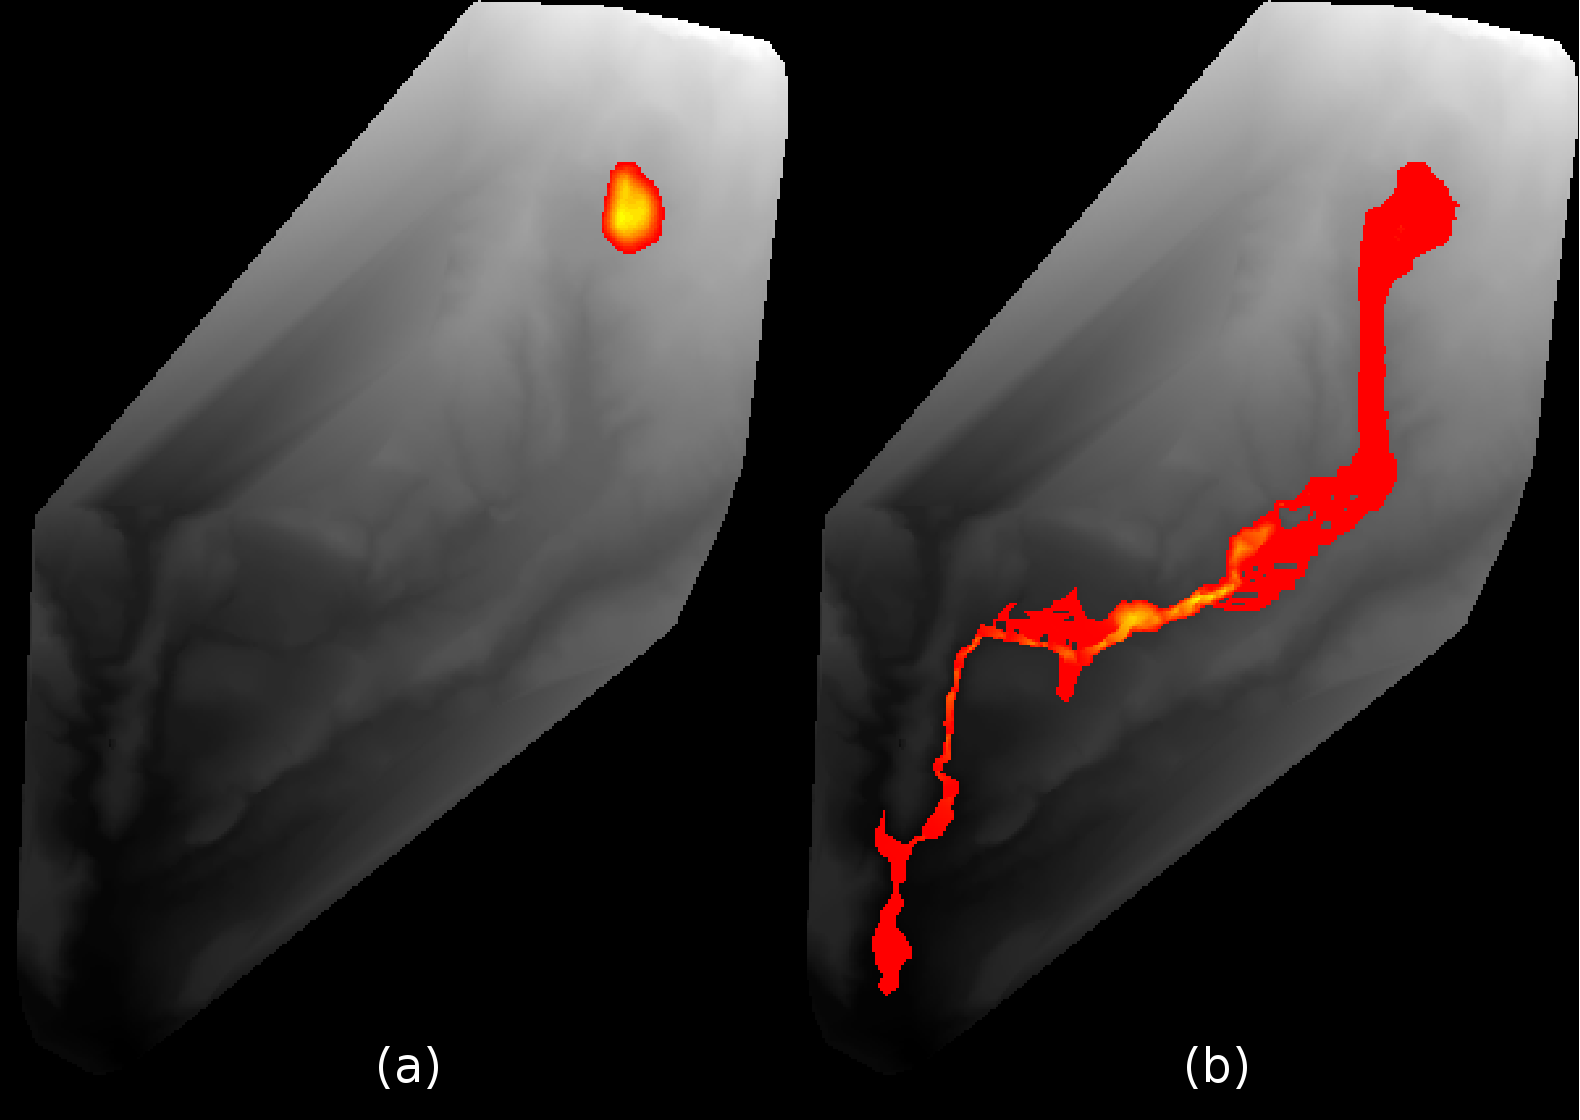
\includegraphics[width=12cm]{./images/OpenCAL/sciddicaT}
  \caption{SciddicaT simulation of the 1992 Tessina (Italy)
    landslide. Topographic altitudes are represented in gray
    scale. Black represents the lower altitude, while the white color
    is used for the highest elevation in the study area. Debris
    thickness is represented with colours ranging from red (for lower
    values) to yellow (for higher values). (a) Initial
    configuration. (b) Final debris flow path. Note that the graphic
    output was generated by using the \texttt{cal\_sciddicaT-glut}
    application, that implements the SciddicaT model and provides a
    minimal visualization system. You can find it in the examples
    directoy.}
  \label{fig:sciddicaT}
\end{figure}

As regards computational preformace, the simulation shown in Figure
\ref{fig:sciddicaT} was executed on a Intel Core i7-4702HQ CPU @
2.20GHz by exploiting only a single core. The simulation lasted a
total of 172 seconds for executing a total of 4000 compuational steps.

Figure \ref{fig:opencal_main_loop} shows the OpenCAL main loop. Before
entering the loop, if defined, the init function is
executed. Afterwards, while the current step is lower or equal to the
final step of computation (or this latter is set to
\verb'CAL_RUN_LOOP'), elementary processes are executed
cocurrently \footnote{On the serial version of OpenCAL, implicit
  parallelism is obtained by exploiting the two different computing
  planes built into OpenCAL's substates. The first one, that we will
  call \emph{current}, is used to read substates's values for the
  central cell and its neighbours, while the second, that we will call
  \emph{next}, is used to update the new state for the central
  cell. When all the cells have been processed and the new state
  values updated, computing planes are switched, i.e. the \emph{next}
  plane is assumed as \emph{current} and the \emph{current} as
  \emph{next}, and the process is reiterated. In this manner, the
  \emph{current} computing plane is not \emph{corrupted} during a
  computational step, being new values written to the \emph{next}
  plane. Note that, even in the case more processing units are used to
  compute the next CA state and more cells are updated simltaneously,
  which is the case of OpenCAL-OMP and OpenCAL-CL, the two computing
  planes are manteined}. In this cycle, substates are updated after
each elementary process has been applyed, while just before the end of
the computational step, if defined, the steering function is
executed. At the end of the computational step, a stop condition is
checked, which can stop the simulation before the last step is
reached. In order to define such a stop condition, the user can use
the \verb'stopCondition()' function, which registers a callback in
which the stop condition can be defined.

\begin{figure}[htbp]
  \centering
  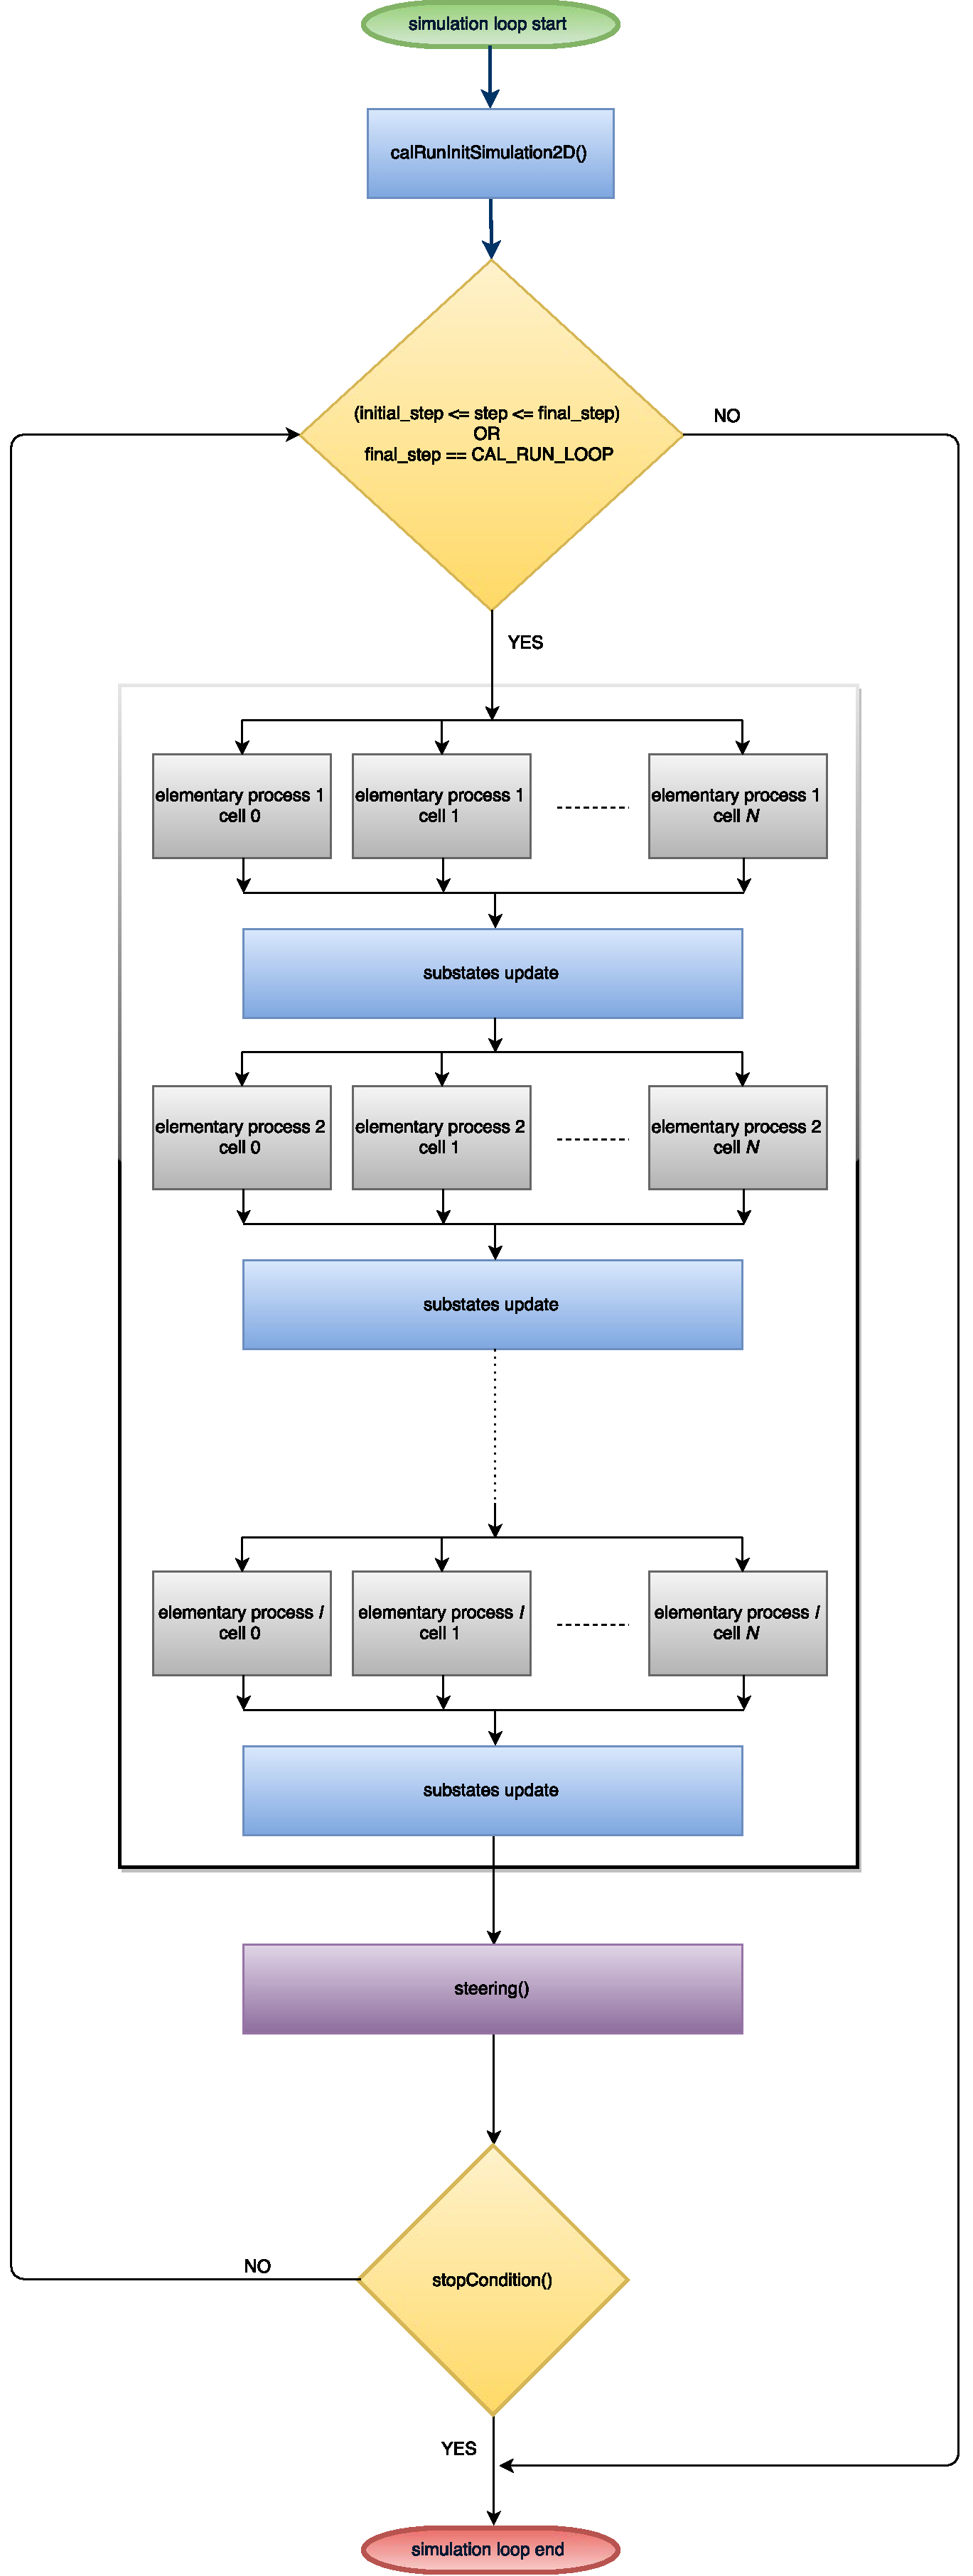
\includegraphics[width=9.5cm]{./images/OpenCAL/opencal_main_loop.pdf}
  \caption{OpenCAL main loop chart.}
  \label{fig:opencal_main_loop}
\end{figure}


\section{SciddicaT with active cells optimization}
Here we present a computationally improved version of SciddicaT, which
takes advantage of the built-in OpenCAL active cells optimization. As
stated above, this optimization is able to restrict computation to a
subset of cells which are actually involved in computation, by
neglecting those cells for which is sure they will not change state to
the next step (stationary cells).

In the case of SciddicaT, only cells containing debris and their
neighbours can change state to the next step, as they can be
interestefd in mass variation due to otflows and inflows. At the
beginning of the simulation, we can simply initialize the set of
active cells to those cells containing debris (i.e. those cells
forming the initial landslide source). Moreover, we can add to this
set new cells or remove some ones from it. Specifically, if an outflow
is computed from an active cell towards a neighbouring stationary
cell, this latter can be added to the set of active cells and
considered for state change by the remaining elementary processes in
the current step of cmputation (if any), or by the next computational
step. Similarly, if a given active cell looses a sufficient amount of
debris, it can be eliminated from the set of active cells. In the case
of SciddicaT, this appens when its thickness becomes lower than or
euqal to a given threshold (i.e. $p_\epsilon$).

In order to account for these processes, we have to slightly revise
the SciddicaT definition. In particular we have to add the set of
active cells, A. The optimized SciddicaT model is now defined as

$$SciddicaT = < R, A, X, Q , P, \sigma >$$
where $A \subseteq R$ is the set of active cells, while the other
components are defned as before. The transition function is now defined as:

$$\sigma : A \times Q^5 \shortrightarrow Q \times A$$ denoting that it
is applied to only the cells in $A$ and that it can add/remove active
cells. More in detail, the $\sigma_1$ elementary process have to
be modified, as it can activate new cell. Moreover, a new elementary
process, $\sigma_3$, have to be added in order to remove cells that
cannot produce outflows during the next computational step due to the
fact that their debris thickness is negligible. The new sequence of
elementary processes is listed below, in the same order they are
applied.

\begin{itemize}
\item $\sigma_1 : A \times (Q_z \times Q_h)^5 \times p_\epsilon \times p_r
  \shortrightarrow Q_o^4 \times A$ determines the outflows from the
  central cell to the neighboring ones, as before. In addition, each
  time an outflow is computed, the neighbour receiving the flow is
  added to the set of active cells.

\item $\sigma_2: A \times Q_h \times (Q_o^4)^4 \shortrightarrow Q_h$ determines
  the value of debris thickness inside the cell by considering mass
  exchange in the cell neighborhood. This elementary process does not
  change with respect to the original version of SciddicaT.

\item $\sigma_3: A \times Q_h \times p_\epsilon \shortrightarrow A$
  removes a cell from $A$ if its debris thickness is lower than or
  equal to the $p_\epsilon$ threshold.
\end{itemize}

In order to implement the SciddicaT debris flows model in OpenCAL by
exploiting the active cells optimization, we have to chage the
definition of the CA objet, by also adding the third $\sigma_3$
elementary process to it. Moreover, the $\sigma_1$ elementary process
have to also be changed. A complete implementation of the sactive
cells optimized version of SciddicaT is shown in Listing
\ref{lst:cal_Sciddicat-activecells} for the sake of completeness, even
if only the differences with respect to the original impleme ntation
are commented.

\lstinputlisting[label=lst:cal_Sciddicat-activecells, caption=An OpenCAL implementation of the SciddicaT debris flows simulation model with the active cells optimization.]{../opencal/OpenCAL/examples/cal_sciddicaT-activecells/source/sciddicaT.c}

%% All of this is done in the \verb'sciddicaTCADef()' function,
%% that you can see in Listing \ref{lst:sciddicaTCADef()}, and on the
%% $\sigma_1$ and $\sigma_3$ elementary processes, that you can find in
%% Listing \ref{lst:sciddica_sigma13}.

%% \begin{lstlisting}[float,floatplacement=H, label=lst:sciddicaTCADef(), caption=The sciddicaTCADef() definition function.]
%%   // define CCA and simulation objects
%%   sciddicaT = calCADef2D (ROWS, COLS, CAL_VON_NEUMANN_NEIGHBORHOOD_2D, CAL_SPACE_TOROIDAL, CAL_OPT_ACTIVE_CELLS);
%%   sciddicaTsimulation = calRunDef2D(sciddicaT, 1, CAL_RUN_LOOP, CAL_UPDATE_IMPLICIT);

%%   // add sigma_1, sigma_2 and sigma_3 elementary processes
%%   calAddElementaryProcess2D(sciddicaT, sciddicaT_flows_computation);
%%   calAddElementaryProcess2D(sciddicaT, sciddicaT_width_update);
%%   calAddElementaryProcess2D(sciddicaT, sciddicaT_remove_inactive_cells);

%%   // add substates
%%   Q.z = calAddSubstate2Dr(sciddicaT);
%%   Q.h = calAddSubstate2Dr(sciddicaT);
%%   Q.f[0] = calAddSubstate2Dr(sciddicaT);
%%   Q.f[1] = calAddSubstate2Dr(sciddicaT);
%%   Q.f[2] = calAddSubstate2Dr(sciddicaT);
%%   Q.f[3] = calAddSubstate2Dr(sciddicaT);

%%   //load configuration
%%   sciddicaTLoadConfig();

%%   //simulation run setup
%%   calRunAddInitFunc2D(sciddicaTsimulation, sciddicaTSimulationInit);
%%   calRunInitSimulation2D(sciddicaTsimulation);
%%   calRunAddSteeringFunc2D(sciddicaTsimulation, sciddicaTSteering);
%%   calRunAddStopConditionFunc2D(sciddicaTsimulation, sciddicaTSimulationStopCondition);
%% \end{lstlisting}


%% Note also that the \verb'calRunInitSimulation2D()' is called at line
%% 23 to initialize the simulation. It simply calls the simulation
%% initialization callback function, that is registered by means of the
%% \verb'calRunAddInitFunc2D()' function at line 22. This is necessary in
%% this example becaouse we don't use here the \verb'calRun2D()'
%% simulation loop, but we make the simulation loop explicit into the
%% idle function of a glut application. If you use the \verb'calRun2D()'
%% function, as we did before, you don't need to call
%% \verb'calRunInitSimulation2D()'.

%% As you can see, besides the CA object, also the definition of the
%% simulation object has changed, being the last step of computation set
%% to \verb'CAL_RUN_LOOP' (line 3). Using such a pre-defined constant
%% determines an infinite loop. As a consequence, the
%% \verb'sciddicaTSimulationStopCondition()' callback has been registered
%% to the simulation object by means of the
%% \verb'calRunAddStopConditionFunc2D()' function (line 25) to stop the
%% simulation\footnote{Such a callback was here introduced to show you
%%   how to define a generic stoppig criterion for the simulation, even
%%   the defined stopping creiterion is very trivial. It simply becomes
%%   true (i.e. the function returns \texttt'CAL\_TRUE', which determines
%%   the end of the simulation loop) when a predefined number of steps is
%%   reached (i.e. 4000, as before).}. The
%% \verb'sciddicaTSimulationStopCondition()' callback function is shown
%% in Listing \ref{lst:sciddicaTSimulationStopCondition()}.


%% \begin{lstlisting}[float,floatplacement=H, label=lst:sciddicaTSimulationStopCondition(), caption=The sciddicaTSimulationStopCondition() callback function defining the simulation stopping criterion for the SciddicaT optimized model.]
%%   CALbyte sciddicaTSimulationStopCondition(struct CALModel2D* sciddicaT)
%%   {
%%     if (sciddicaTsimulation->step >= STEPS)
%%       return CAL_TRUE;
%%     return CAL_FALSE;
%%   }
%% \end{lstlisting}


%% \begin{lstlisting}[float,floatplacement=H, label=lst:sciddica_sigma13, caption=The $\sigma_1$ and $\sigma_3$ SciddicaT elementary processes with active cells optimization.]
%%   // <snip>

%%   // The sigma_1 elementary process
%%   void sciddicaT_flows_computation(struct CALModel2D* sciddicaT, int i, int j)
%%   {
%%     // <snip>
    
%%     for (n=1; n<sciddicaT->sizeof_X; n++)
%%       if (eliminated_cells[n])
%%         calSet2Dr(sciddicaT, Q.f[n-1], i, j, 0.0);
%%       else
%%       {
%%         calSet2Dr(sciddicaT, Q.f[n-1], i, j, (average-u[n])*P.r);
%%         calAddActiveCellX2D(sciddicaT, i, j, n);
%%       }
%%   }

%%   // <snip>
  
%%   // The sigma_3 elementary process
%%   void sciddicaT_remove_inactive_cells(struct CALModel2D* sciddicaT, int i, int j)
%%   {
%%     if (calGet2Dr(sciddicaT, Q.h, i, j) <= P.epsilon)
%%       calRemoveActiveCell2D(sciddicaT,i,j);
%%   }

%%   // <snip>
%% \end{lstlisting}


%% The complete source code of the optimized version of SciddicaT can be
%% found in OpenCAL examples under the name
%% \verb'cal_sciddicaT-activecells-glut'.

As you can easily see, few modifications to the original source code
are needed to add the active cells optimization to SciddicaT. In
particular, the active cells optimization is enableb by means of the
\verb'CAL_OPT_ACTIVE_CELLS' parameter at line 159, while the third
elementary process added at line 165. As regards the elementary
processe $\sigma_1$, it is the same of the one of the basic SciddicaT
version, with the exception that when an outflow is generated, the
cell receiving the flow is added to the set A of the active cells
(line 88). Moreover, an active cell is eliminated by the set A by
means of the $\sigma_3$ elementary process in the case its debris
thickness becomes lower than or equal to the $P_\epsilon$ threshold
parameter (lines 107-108).

Regarding the computational preformace, the same simulation shown in
Figure \ref{fig:sciddicaT} was executed using the new SciddicaT
implementation adoptig the active cells implementation. Still, only a
single core of the same Intel Core i7-4702HQ CPU was used, as we did
before. The simulation lasted a total of 22 seconds, versus 172
seconds obtained for the basic (non-optimized) version, whihc is about
8 times faster. Given the small required implementatice effort, we
think it can be condidered a very good result.

\section{SciddicaT as eXtended CA}
OpenCAL allows for further optimization of the SciddicaT debris flows
simulation model by means of the so called \emph{unsafe
  operations}. In fact, in some cases, it is possible to consider an
extended definition of the computational model, allowing for
operations that are not strictly permitted by the formal definition of
Cellular Automata. In particular, we will allow the transition
function to update the state of the neighbouring cells, while the CA
only allows for state change for of the central one. When we will
permit such a kind of unsafe operations, we will talk about \emph{XCA
  eXtended Cellular Automata}. Obviously, the extended CA must be
equivalent to the original one in terms of computational results.

An XCA equivalent version of SciddicaT can be obtained by obseving
that, when an outflow is computed from the central cell towards a
neighbour, the flow can be immediatly subtracted from the central cell
and added to the neighbour. This does not change the state of the
system at the current step, which is represented by means of the
\emph{current} computational plane, as updated values are written to
the \emph{next} plane. Thus, the \emph{current} computational plane is
not corrupted by the extended operation, while the \emph{next} plane
is used for immediatly accounting mass variations inside the cells. By
introducing such feature, ouflows don't need to be saved into otflows
substates anymore, as they are used to account mass exchange directly
during ouflows computation. As you can figure out, this can give rise
to a further performace improvement of the application. The SciddicaT
XCA model is formally defined as:


$$SciddicaT = < R, A, X, Q , P, \sigma  >$$

where:

\begin{itemize}

\item $R$ is the set of points, with integer coordinates, which
  defines the 2-dimensional cellular space over which the phenomenon
  evolves. The generic cell in $R$ is individuated by means of a
  couple of integer coordinates $(i, j)$, where $0 \leq i < i_{max}$
  and $0 \leq j < j_{max}$. The firt coordinate, $i$, represents the
  row, while the second, $j$, the column. The cell at coodinates
  $(0,0)$ is located at the top-left corner of the computational grid.

\item $A \subseteq R$ is the set of active cells, i.e. those cells
  actually involved in computation.

\item $X = \{(0,0), (-1, 0), (0, -1), (0, 1), (1, 0)\}$ is the von
  Neumann neighborhood relation, a geometrical pattern which
  identifies the cells influencing the state transition of the central
  cell. The neighborhood of the generic cell of coordinate $(i, j)$ is
  given by
$$N(X, (i, j)) =$$
$$= \{(i, j)+(0,0), (i, j)+(-1, 0), (i, j)+(0, -1),
(i, j)+(0, 1), (i, j)+(1, 0)\} =$$
$$= \{(i, j), (i-1, j), (i, j-1), (i, j+1), (i+1, j)\}$$

Here, a subscript operator can be used to index cells belonging to the
neighbourhood. Let $|X|$ be the number of elements in X, and $n \in
\mathbb{N}$, $0 \leq n < |X|$; the notation

$$N(X, (i, j), n)$$

represents the $n^{th}$ neighbourhood of the cell $(i,j)$. Thereby, $N(X, (i, j), 0) = (i, j)$, i.e. the central cell, $N(X, (i, j), 1) = (i-1, j)$, i.e. the first neighbour, and so on.

\item $Q$ is the set of cell states; it is subdivided in the following
  substates:

\begin{itemize}
    \item   $Q_z$ is the set of values representing the topographic altitude (i.e. elevation);
    \item   $Q_h$ is the set of values representing the debris thickness;
\end{itemize}

The Cartesian product of the substates defines the overall set of
state $Q$:

$$Q = Q_z \times Q_h$$
so that the cell state is specified by:

$$ q = (q_z, q_h)$$

\item   $P$ is set of parameters ruling the CA dynamics:

\begin{itemize}
    \item   $p_\epsilon$ is the parameter which specifies the thickness of the debris that cannot leave the cell due to the effect of adherence;
    \item   $p_r$ is the relaxation rate parameter, which affects the size of outflows (cf. section above).
\end{itemize}

\item $\sigma : A \times Q^5 \shortrightarrow Q$ is the deterministic cell
  transition function. It is composed by two elementary processes:
\begin{itemize}
\item $\sigma_1 : A \times (Q_z \times Q_h)^5 \times p_\epsilon \times
  p_r\shortrightarrow (A \times Q_h)^5$ determines the outflows from
  the central cell to the neighboring ones and updates debris
  thickness inside the central cell and its neighbours accordingly. It
  also adds the neighbouring cells receining a flow to the set A of the
  active cells.

\item $\sigma_2: A \times Q_h \times p_\epsilon \shortrightarrow A$ removes the
  cell from the set A of the active cells if the debris thickness
  inside the cell is lower than or equal to the $p_\epsilon$
  threshold.

\end{itemize}
\end{itemize}

Note that, only the topographic altitude and the debris thicness are
now considered as model's substates, as the four outflows substates
are no longer needed. Moreover, the number of elementary process now
considered is two, instead of three for the previous versions of
SciddicaT. The OpenCAL implementation of the further optimized
SciddicaT debris flows model is shown in Listing
\ref{lst:cal_sciddicaT-unsafe}.

\lstinputlisting[label=lst:cal_sciddicaT-unsafe, caption=An OpenCAL implementation of the SciddicaT further optimized debris flows simulation model.]{../opencal/OpenCAL/examples/cal_sciddicaT-unsafe/source/sciddicaT.c}

As you can see, the definitions of CA and simulation objects doesn't
change from the previous implementation (lines 131-132), while only
two elementary processes are considered (lines 135-136). In
particular, the firt call to \verb'calAddElementaryProcess2D()'
registers the callbak function implementing the $\sigma_1$ elementary
process. It computes outflows from the (active) central cell to its
neighbours (line 83) and updates the debris tickness in both the
central cell and the neighbouring cell receiving a flow (lines
84-85). Moreover, neighbouring cells receiving a flow are added to the
set A of active cells (line 88) and therefore will be considered for
elaboration by the subsuequent elementary process ($\sigma_2$) in the
current step of computation\footnote{This is due to the fact that a
  substates' update is performed after the first elementary process
  has been applied to all the (active) cells of the cellular
  space. This behaviour is set by menas of the
  \texttt{CAL\_UPDATE\_IMPLICIT} parameter used in the definition of
  the simulation object at line 132 of Listing
  \ref{lst:cal_sciddicaT-unsafe}.} and, if it is not removed by
$\sigma_2$), by the subsequent computational steps. In particular, the
\verb'calSetX2Dr()' \emph{unsafe} function is used to update the
derbis thickess of the neighbouring cells receiving a flow, while the
\verb'calAddActiveCellX2D()' function is used to add a neighbouring
cells receiving a flow to the set $A$ of active cells.  The $\sigma_2$
elementary process, simply remove inactive cells from $A$ (lines
95-86), as in the previous example.


Substates are added to the CA at lines 139-140. Here, note that the
firt substate, $Q_z$, is added by menas of the
\verb'calAddSingleLayerSubstate2Dr()' function. It is here considered
to allocate memory only for the \emph{current} computing plane. In
fact, topographic altitutde only changes at the simulation
initialization stage (cf. lines 147 and 117), while it remains
inalterated during computation as its value is never updated by the
transition function. This allows for memory space allocation
optimization and possibly for computational performance
improvements. Note that, at line 117 we used the
\verb'calSetCurrent2Dr()' function, instead of the usual
\verb'calSet2Dr()'. The \verb'calSetCurrent2Dr()' function  allows for updating the \emph{current} computational plane (the only present in the $Q_z$ substate), while \verb'calSet2Dr()' would update the \emph{next}
computational plane, by producing an access violation error.

Regarding the computational preformace, the same simulation shown in
Figure \ref{fig:sciddicaT} was executed by considering the XCA
implementation of SciddicaT on a single core of the same
processor. The simulation lasted a total of 11 seconds, versus 22
seconds obtained for the active cells optimized version and 172
seconds for the basic (non-optimized) version. The XCA implementation resulted 2 times
faster than the active cells optimized version and about 16 times faster with
than the basic one.



\section{SciddicaT with explicit simulation loop}
Even if results obtained so far are more than satisfying, it is
further possibile to improve computational performance of SciddicaT by
avoiding unnecessary substates updating. In fact, in some cases, elementary
processes don't affect one or more model's substates and therefore their
updating becomes only a waste of time.

As we stated above, when we use the implicit \verb'calRun2D()'
simulation loop, an update of all the defined substates is executed at
the end of each elementary process. However, this behaviour can be
changed by making the OpenCAL simulation loop explicit.

In the specific case of the SciddicaT XCA model, the second elementary
process, $\sigma_2$, just remove cells that became inactive from the
set $A$ of active cells and don't affect the mode's
substates\footnote{Actually, only the $Q.h$ substate can be update by
  the transition function, since the other, $Q.z$, is of single-lyer
  type.}. As a consequence, no substates updating should be executed
after $\sigma_2$ application, in order to avoid unnecessary
operations.

A new OpenCAL implementation of SciddicaT is presented in Listing
\ref{lst:cal_sciddicaT-explicit}. It is based on an explicit
simulation loop and also defines a stopping criterion for the
simulation termination. The complete implementation is shown for the
sake of completeness.


\lstinputlisting[label=lst:cal_sciddicaT-explicit, caption=An OpenCAL implementation of the SciddicaT XCA debris flows simulation model with explicit simulation loop.]{../opencal/OpenCAL/examples/cal_sciddicaT-unsafe-explicit/source/sciddicaT.c}


As you can see, the \verb'calRunAddGlobalTransitionFunc2D()' function
is called to register a custom transition function (line 177). In the
specific case of SciddicaT, the \verb'sciddicaTransitionFunction()'
callback (lines 132-143) is used to make the elementary processes
application and the substates update explicit. Here, the elementary
processes are applyied in the same order they are defined (which is
the default behaviour of OpenCAL). In particular, the
\verb'sciddicaT_flows()' elementary process is applyied to each
(active) cell into the computational domain by means of the
\verb'calApplyElementaryProcess2D()' function. After that, the set $A$
of the active cells and the $Q_h$ substate are updated by means of the
\verb'calUpdateActiveCells2D()' and \verb'calUpdateSubstate2Dr()',
respectively.



Table \ref{tab:speedup} resumes the
computational performace of the above illustraed versions of
SciddicaT.

\begin{table}
  \centering
  \begin{tabular}{l|c|c}
    \hline
    CA model & Elapsed time [s] & Speedup \\
    \hline
    \hline
    SciddicaT                   & 240 & 1\\
    SciddicaT with active cells & 23  & 10.43\\
    SciddicaT XCA (eXtended CA) & 13  & 18.46\\
    SciddicaT XCA explicit loop & 12  & 20\\
    \hline
  \end{tabular}
  \caption{Computational performace of the four different
    implementations of the SciddicaT debris flows model.}
  \label{tab:speedup}
\end{table} 


\section{A three-dimensional example}

In order to introduce you to development with of three-dimensional CA
with OpenCAL, we start this section by implementing a simple 3D model,
namely the mod2 3D CA. Cells can be in one of two differnt states, 0
or 1, as in Game of Life. The cellular space is a parallelepiped made
by cubic cells, while the cell's neighbourhood is the 3D Moore one,
consisting of the central cell and its adjecent cells. The transition
function simply evaluates the quantity $s$ as the number of
neighbouring cells which are in the state 1 and sets the new state for
the central cell as $s\%2$.

$$mod2 = < R, X, Q, \sigma >$$

where:

\begin{itemize}

\item $R$ is the set of points, with integer coordinates, which
  defines the 3-dimensional cellular space. The generic cell in $R$ is
  individuated by means of a triple of integer coordinates $(i, j,
  k)$, where $0 \leq i < i_{max}$, $0 \leq j < j_{max}$, and $0 \leq k
  < k_{max}$. The firt coordinate, $i$, represents the row, the
  second, $j$, the column, while the third coordinate represents the
  slice. The cell at coodinates $(0,0,0)$ is located at the
  top-left-far corner of the computational grid.

\item $X = \{(0,0,0), \dots, (-1,1,0), (0,0,-1), \dots, (-1,1,-1),
  (0,0,1), \dots, (-1,1,1)\}$ is the Moore neighborhood
  relation, a geometrical pattern which identifies the cells
  influencing the state transition of the central cell. The
  neighborhood of the generic cell of coordinate $(i, j)$ is given by
  $$N(X, (i, j, k)) = $$
  $$= \{(i, j, k)+(0,0,0), \dots, (i, j, k)+(-1,1,-1)\} =$$
  $$= \{(i, j, k), \dots, (i-1,j+1,-1)\}$$
  Here, a subscript operator can be used to index cells belonging to the
  neighbourhood. Let $|X|$ be the number of elements in X, and $n \in
  \mathbb{N}$, $0 \leq n < |X|$; the notation

  $$N(X, (i, j), n)$$

  represents the $n^{th}$ neighbourhood of the cell $(i,j)$. Thereby,
  $N(X, (i, j, k), 0) = (i, j, k)$, i.e. the central cell, $N(X, (i, j, k), 1)
  = (i-1, j, k)$, i.e. the first neighbour, and so on.
  
\item $Q = \{0, 1\}$ is the set of cell states.
  
\item $\sigma : Q^{27} \shortrightarrow Q$ is the deterministic cell
  transition function. It is composed by one elementary process, which
  implements the previously descripted transition rules.
\end{itemize}


As you can imagine, the OpenCAL implementation of the mod2 3D CA is
very simple, as the Conway's game of Life is. The complete source code
is shown in Listing \ref{lst:cal_mod2CA3D}.

\lstinputlisting[label=lst:cal_mod2CA3D, caption=An OpenCAL implementation of the mod2 3D CA.]{../opencal/OpenCAL/examples/cal_mod2CA3D/source/mod2CA3D.c}

As you can see, even if Listing \ref{lst:cal_life} is very short, it
completely defines the mod2 3D CA and perform a simulation (actually,
only one step in this example). Lines 3-5 include some header files
for the 3D version of OpenCAL, while lines 12-14 declare CA, substate
and simulation objects. They are therefore defined later in the main
function. In particular, line 30 defines the CA as a parallelepiped
having \verb'ROWS' rows, \verb'COLS' columns and \verb'SLICES' slices
(cf. lines 7-9). Moreover, the 3D Moore neighbourhood is here set as
well as cyclic conditions at boundaries. Eventually, no optimizations
are considered. Line 31 defines the simulation object by setting just
one step of computation and implicit substate's update. Finally, the
only substate, $Q$, is defined at line 34. Note that, since it was
defined by means of the \verb'calInitSubstate3Db()' function, each
element $q \in Q$ results to be of the CALbyte type. Line 37 registers
the only CA's elementary process, namely the
\verb'mod2_transition_function()' function, which is then implemnented
at lines 17-25. Line 43 initializes the cell's substated $Q$ at
coordinates (2, 3, 1) to the state 1. The obtained initial
configuration is then saved to disk at line 46, and the simulation ran
at line 49. The final configuration is therefore saved to disk at line
52 and, eventually, memory previously and implicitly allocated is
released at lines 55-56. Note that, diffrently to the previous
examples, almost all the OpenCAL functions come in the 3D flower. For
instace, this is the case of the \verb'alGetX3Db()' and
\verb'calSet3Db()' functions at lines 22 and 24, respectively, which
that take the \verb'k' parameter inorder to specify the slice
coordinate for the cell.

Figures \ref{fig:mod2_0000} and \ref{fig:mod2_LAST} show the initial and final configuration of mod2 3D CA as implemented in Listing \ref{lst:cal_mod2CA3D}, respectively.

\begin{figure}
  \begin{center}
    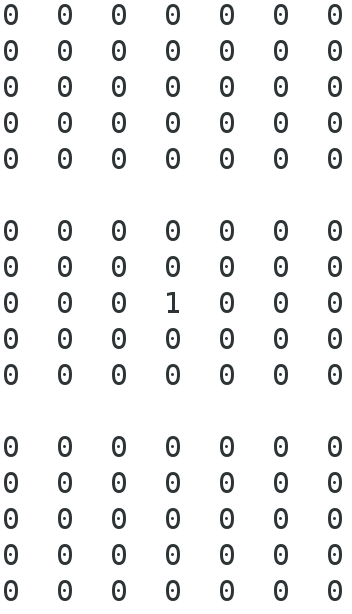
\includegraphics[width=3.5cm]{./images/OpenCAL/mod2_0000}
    \caption{Initial configuration of mod2 3D CA, as implemented in Listing \ref{lst:cal_mod2CA3D}.}
    \label{fig:mod2_0000}
  \end{center}
\end{figure}

\begin{figure}
  \begin{center}
    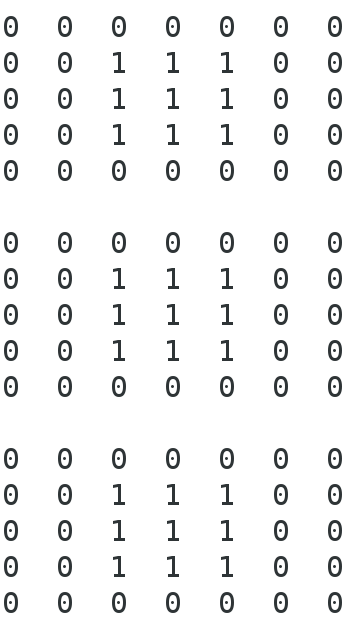
\includegraphics[width=3.5cm]{./images/OpenCAL/mod2_LAST}
    \caption{Final configuration of mod2 3D CA (actually, just one step of computation), as implemented in Listing \ref{lst:cal_mod2CA3D}.}
    \label{fig:mod2_LAST}
  \end{center}
\end{figure}


\begin{figure}
  \begin{center}
    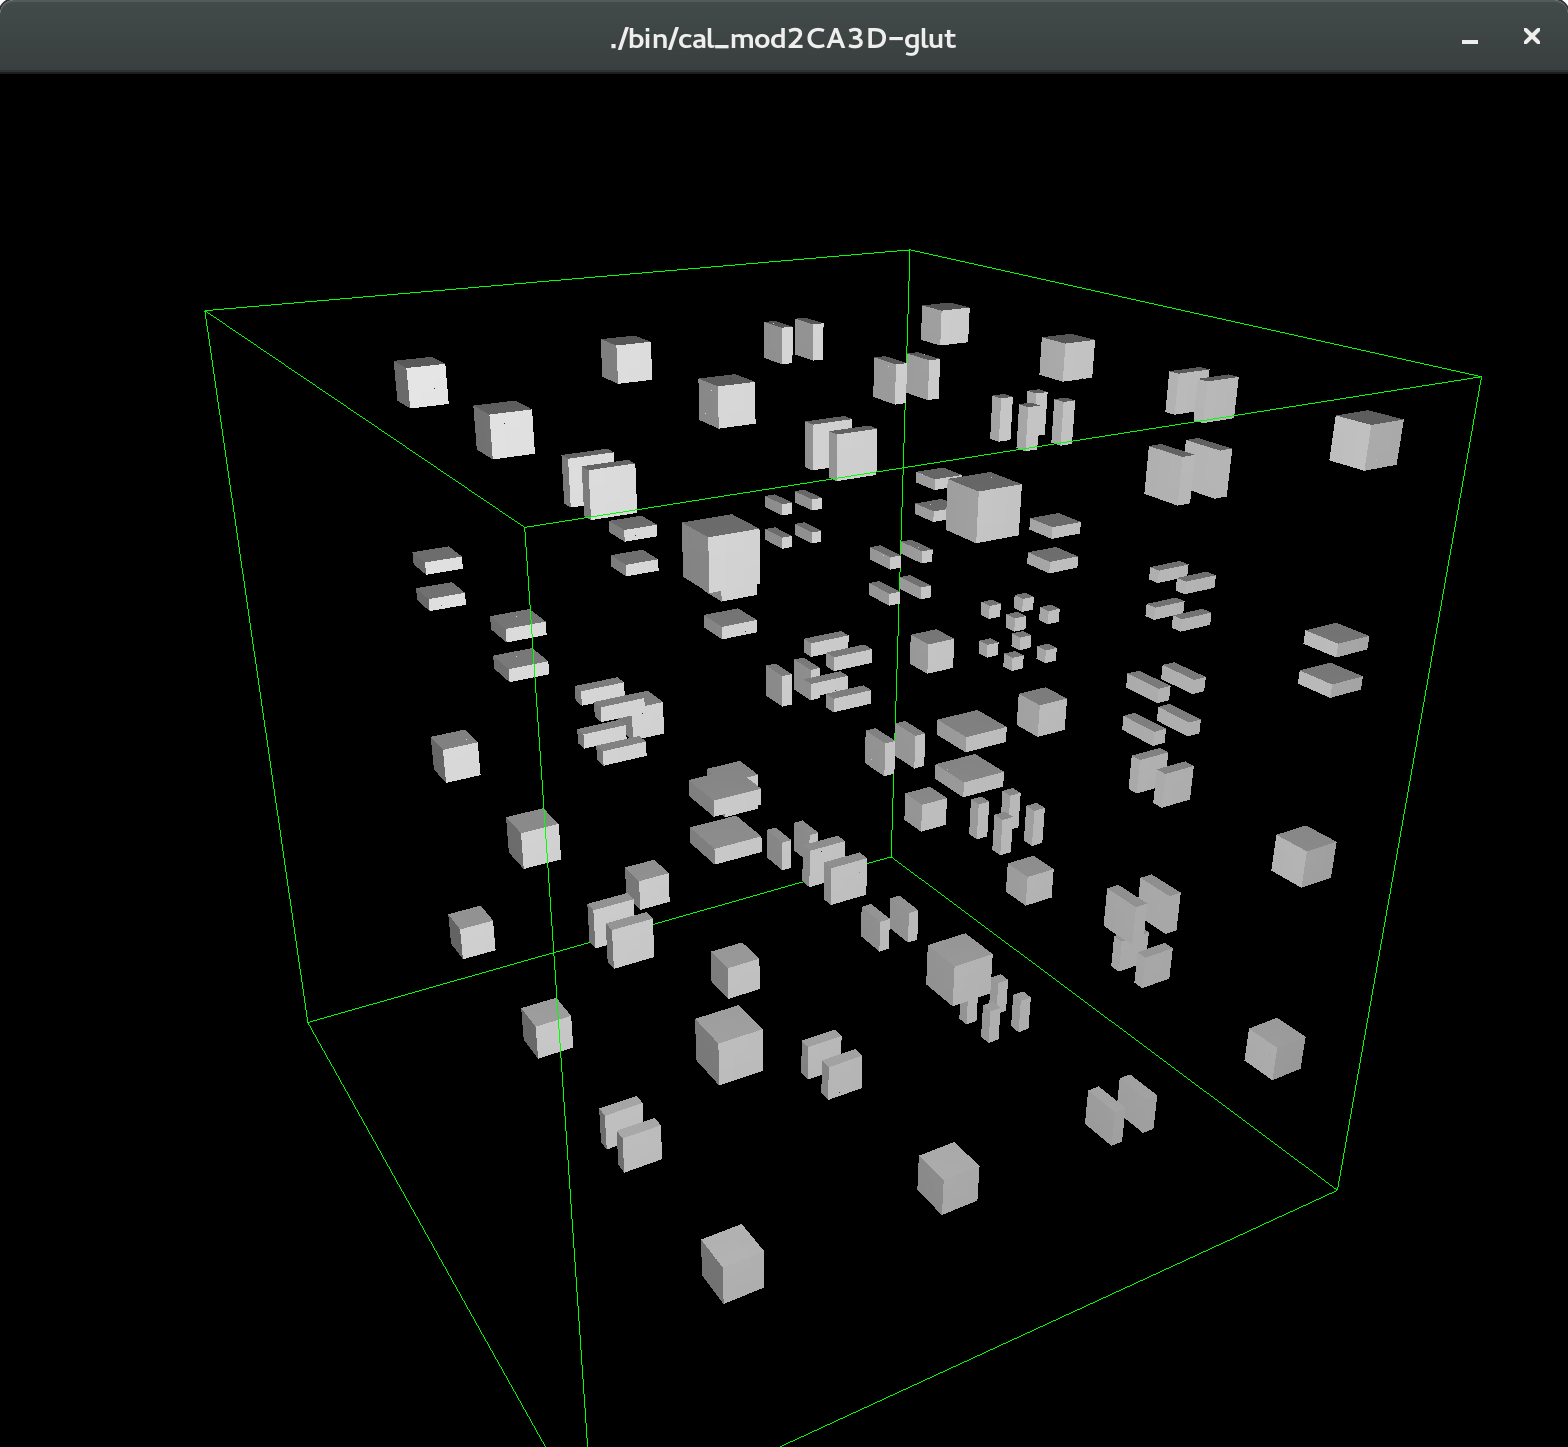
\includegraphics[width=12cm]{./images/OpenCAL/mod23DCA-glut}
    \caption{Graphical representation of the mod2 3D CA after 77 computational steps, as implemented in Listing \ref{lst:cal_mod2CA3D}. CA dimensions were set to (rows, cols, slices) = (65, 65, 65), while the initial seed located at coordinates (12, 12, 12). Cells in black are in the state 0, cell in white are in the state 1.}
    \label{fig:mod2_LAST}
  \end{center}
\end{figure}


\section{Custom Neighbourhoods}
xxx
